\documentclass{beamer}

\usepackage{polski}
\usepackage[utf8]{inputenc}
\usepackage{color}
\usepackage{amsfonts}	% Real

\usepackage{booktabs} % eleganckie tabelki


\usetheme{boxes}      % Wybór tematu wyglądu, gdy chcemy inny
%\usecolortheme{rose}   % Wybór tematu kolorystycznego, j.w.

%Konfiguracja dla pakietu hyperref:
\hypersetup{
  unicode=true,           % włączenie wyświetlania pliterek w zakładkach
%  pdfpagemode=FullScreen, % włączenie trybu pełnoekranowanego
  pdfsubject=Graph Neural Networks,      % temat prezentacji
  pdfkeywords={gnn, graph neural network, graph, classification} % slowa kluczowe
}

%% Dane do strony tytułowej
\author{Aleksy Barcz\\mgr inż. Zbigniew Szymański\\ dr inż. Stanisław Jankowski}
\title{Implementation aspects of\\Graph Neural Networks}
\date{\today}
\institute{Warsaw University of Technology}

\setbeamercovered{transparent}

\begin{document}
\frame{\titlepage}

\begin{frame}
\frametitle{What is a Graph Neural Network?}
\begin{itemize}
	\item Classifier of graphs
	\item \emph{Scarselli et al., 2009}
	\item Most graph types, including nonpositional and cyclic
	\item Node/Graph classification
	\item Based on simple FNN units
	\item Similar to Graph Machines with a different processing schema
\end{itemize}
\end{frame}

\begin{frame}
\frametitle{GNN tasks}
\begin{itemize}
	\item Build representation of graph nodes
	\item Learn to classify them properly
\end{itemize}
\end{frame}

\begin{frame}
\frametitle{Building node representation - $f_w$}
\begin{columns}
	\begin{column}{0.2\textwidth}
		\begin{center}
			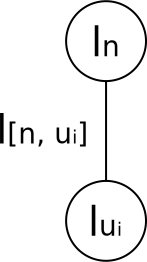
\includegraphics[scale=0.4]{img/connection}
		\end{center}
	\end{column}
	\begin{column}{0.8\textwidth}
		\begin{center}
			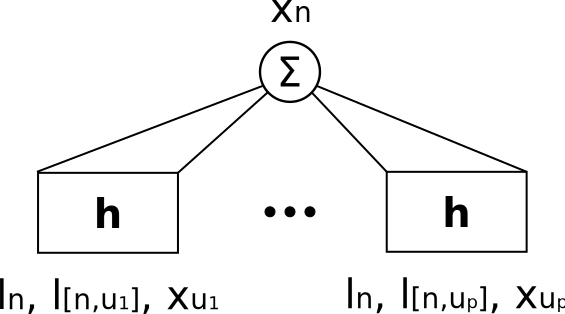
\includegraphics[scale=0.4]{img/f}
		\end{center}
	\end{column}
\end{columns}
\medskip
\begin{itemize}
	\item for node $n$ we consider all nodes $u$ with edge: $u \Rightarrow n$
	\item $h_w$ : FNN (inputs, $tanh$ layer, $tanh$ layer)
\end{itemize}
\end{frame}

\begin{frame}
\frametitle{Node classification - $g_w$}
\begin{center}
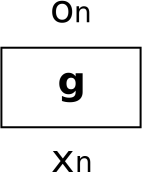
\includegraphics[scale=0.4]{img/g}
\end{center}
\begin{itemize}
	\item $g_w$ takes as input representation of node $n$ : $x_n$, built by $f_w$
	\item $g_w$ : FNN (inputs, $tanh$ layer, $tanh$/$linear$ layer)
\end{itemize}
\end{frame}

\begin{frame}
\frametitle{Encoding network}
\begin{center}
	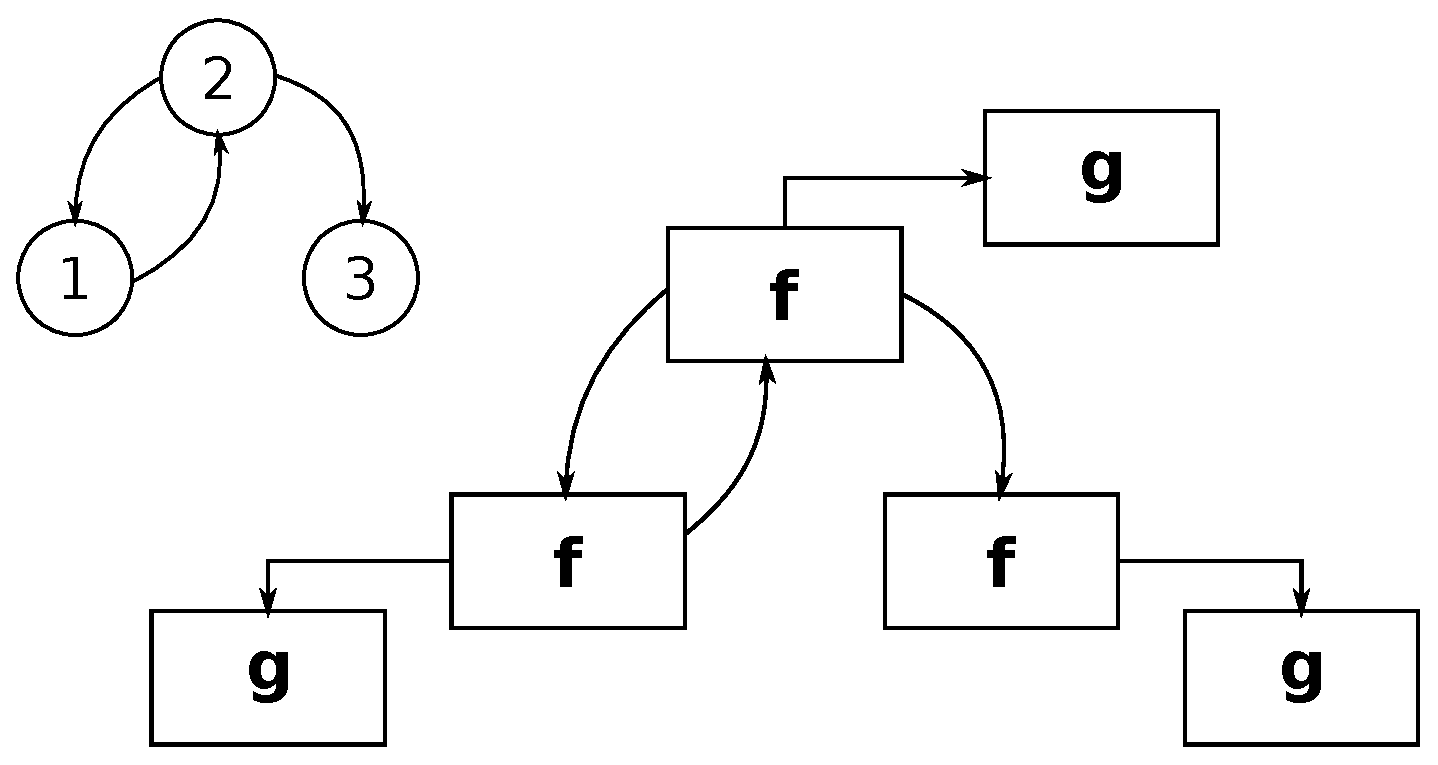
\includegraphics[scale=0.4]{img/encodinginc}
\end{center}
\begin{itemize}
	\item Building node representation: $x_n = f(...)$
	\item Node classification: $o_n = g(x_n)$
	\item All instances of $f_w$ share weights
	\item All instances of $g_w$ share weights
\end{itemize}
\end{frame}

\begin{frame}
\frametitle{Learning algorithm}
\begin{enumerate}
	\item initialize randomly $h_w$ and $g_w$ weights
	\item until stop criterion is satisfied:
	\begin{itemize}
		\item random initialization of representation $X$
		\item FORWARD : calculate $X = F_w(X)$ until fixed point is reached
		\item BACKWARD : calculate $G_w(X)$ and backpropagate the error
		\item update $f_w$ and $g_w$ weights
	\end{itemize}
\end{enumerate}
\end{frame}

\begin{frame}
\frametitle{Forward - building representation}
\begin{columns}
	\begin{column}{0.66\textwidth}
		\includegraphics[scale=0.4]{img/forward2}
	\end{column}
	\begin{column}{0.34\textwidth}
		\begin{itemize}
			\item unfolding
		\end{itemize}
	\end{column}
\end{columns}
\end{frame}

\begin{frame}
\frametitle{Backward - backpropagation}
\begin{columns}
	\begin{column}{0.66\textwidth}
		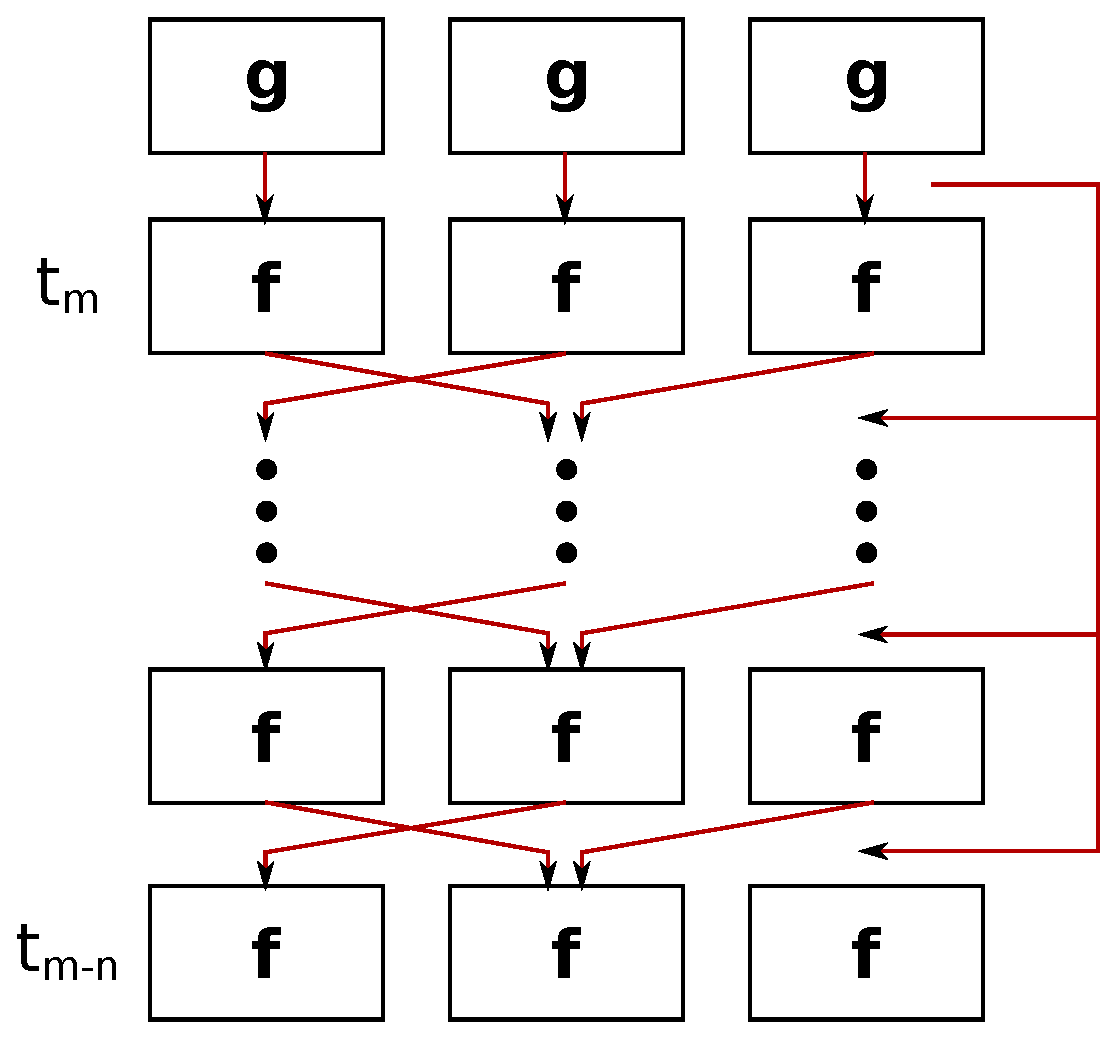
\includegraphics[scale=0.4]{img/backward2}
	\end{column}
	\begin{column}{0.34\textwidth}
		\begin{itemize}
			\item BPTT
			\item Almeida-Pineda
		\end{itemize}
	\end{column}
\end{columns}
\end{frame}

\begin{frame}
\frametitle{How do we know $F_w$ will reach fixed point?}
\begin{itemize}
	\item contraction map (Banach theorem)
	\item $||F_w(X_1) - F_w(X_2)|| \leq ||X_1 - X_2||$
	\item unique fixed point
	\item fixed point reached from every starting point
	\item very few iterations needed
	\item penalty imposed on $F_w$ weights when the contraction is lost
\end{itemize}
\end{frame}

\begin{frame}
\frametitle{How strong should the penalty be?}
\begin{center}
	\includegraphics[scale=0.065]{img/rmse1_clipped}
\end{center}
\begin{itemize}
	\item $contractionConstant \in [1.2, 0.9, 0.6]$
	\item boundary value depends on dataset
\end{itemize}
\end{frame}

\begin{frame}
\frametitle{Results - 5fold crossvalidation, subgraph matching}
\setlength{\tabcolsep}{2pt}
\begin{table}[h!]
	\begin{center}
	\begin{tabular}{llll}
	\toprule
	& accuracy & precision & recall \\
	\midrule
	GNN - tr &	91\% &  87\%&  97\% \\
	GNN - tst &	91\% &  86\% &  97\% \\
	\bottomrule
	\end{tabular}
	\caption{Mean values - GNN}
	\end{center}
\end{table}

\begin{table}[h!]
	\begin{center}
	\begin{tabular}{llll}
	\toprule
	& accuracy & precision & recall \\
	\midrule
	FNN - tr &	71\% &  65\% & 93\% \\
	FNN - tst &	71\% &  64\% &  93\% \\
	\bottomrule
	\end{tabular}
	\caption{Mean values - FNN}
	\end{center}
\end{table}
\end{frame}

\end{document}
